% \begin{frame}{Runwise Plots}
%     \begin{itemize}
%         \item Various changes during runs
%         \item NTracks/Lumi
%         \item Nevent/Lumi
%     \end{itemize}
% \end{frame}

\begin{frame}{2024 Runs Splits}
    \begin{itemize}
        \item Due to the higher backgrounds FaserNu had to be replaced every 10 ifb.
        \item The replacement schedule was as follows
    \end{itemize}
    \begin{table}[h!]
        \begin{tabular}{|l|c|c|c|}
            \hline
            \textbf{Box}  & \textbf{Installed} & \textbf{Removed} & \textbf{Lumi (ifb)} \\ \hline
            F241          & 20/3               & 6/5              & 11.6                \\ \hline
            Tungsten only & 6/5                & 12/6             & 18.5                \\ \hline
            F242          & 12/6               & 8/7              & 9.9                 \\ \hline
            CaloNu        & 10/7               & 4/10             & 69.8                \\ \hline
            F243          & 4/10               & 22/10            & 11.9                \\ \hline
        \end{tabular}
        \caption{Replacement Schedule [Source: \href{https://indico.cern.ch/event/1350805/contributions/5686417/attachments/2963344/5212652/FASER-GeneralMtg-8.11.24.pdf}{FASER General Meeting 8.11.24}]}
    \end{table}
\end{frame}

\begin{frame}{Runwise Plots of 2023}
    \begin{figure}
        \centering
        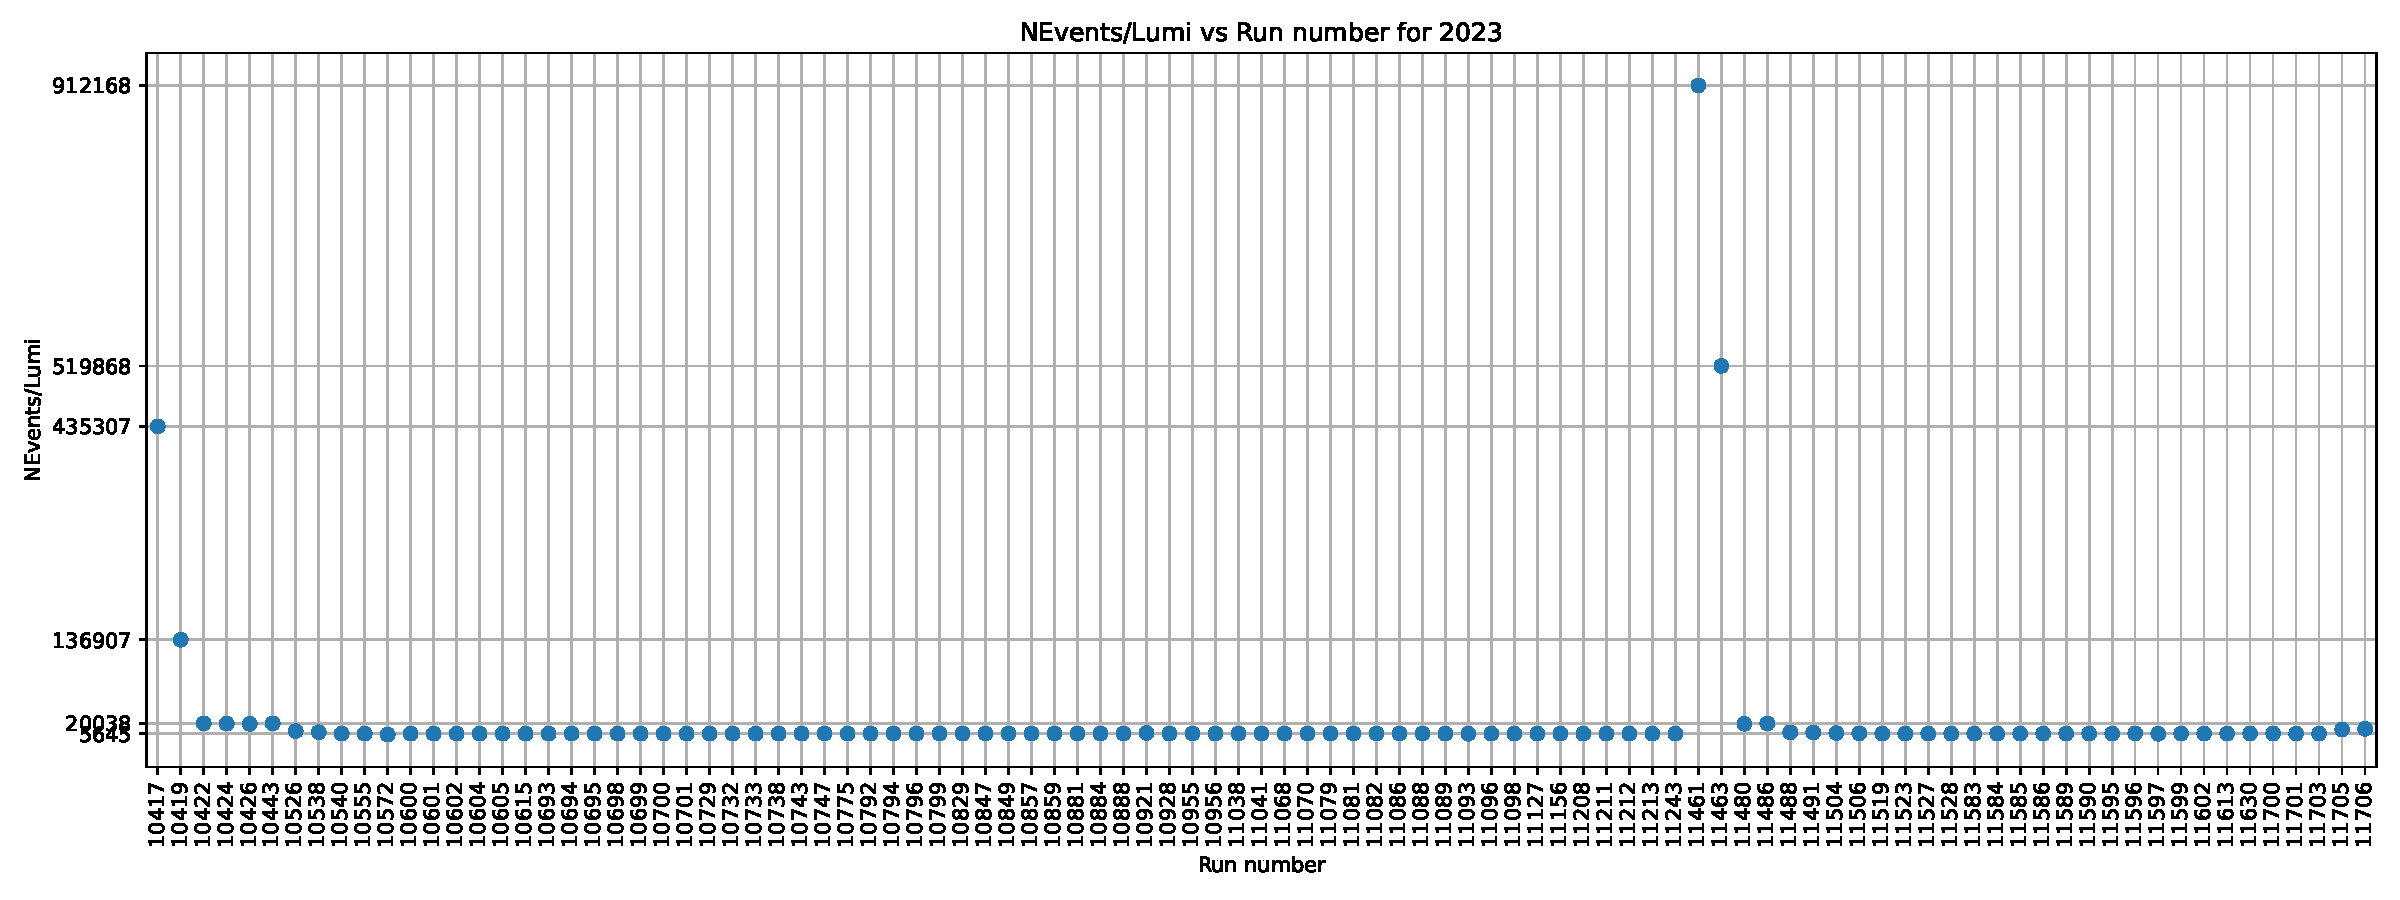
\includegraphics[width=1.0\textwidth]{plots_runwise/NEventsbyLumi_2023.pdf}
    \end{figure}
    \vspace{-0.35cm}
    \begin{figure}
        \centering
        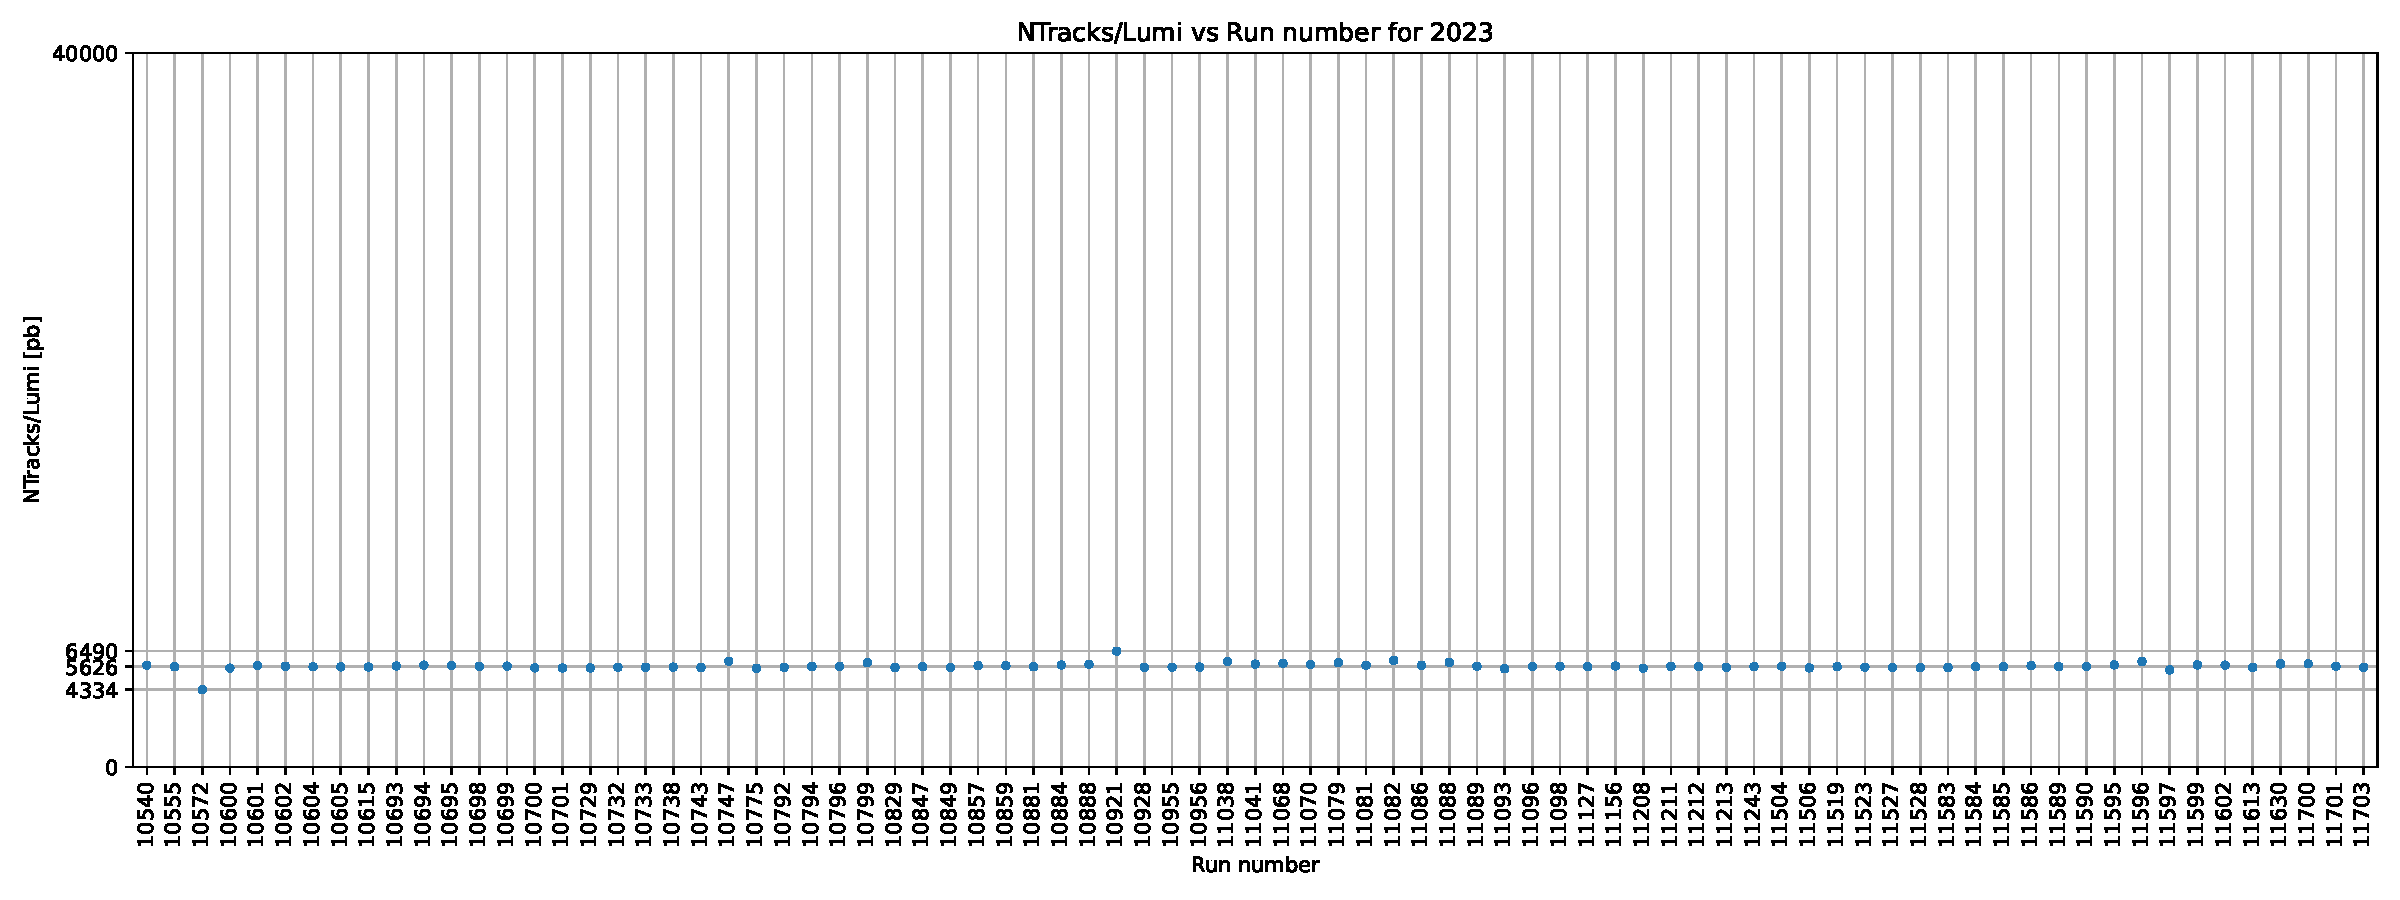
\includegraphics[width=1.0\textwidth]{plots_runwise/NTracksbyLumi_2023.pdf}
    \end{figure}
\end{frame}



\begin{frame}{Runwise Plots of F241- 2024}
    \begin{figure}
        \centering
        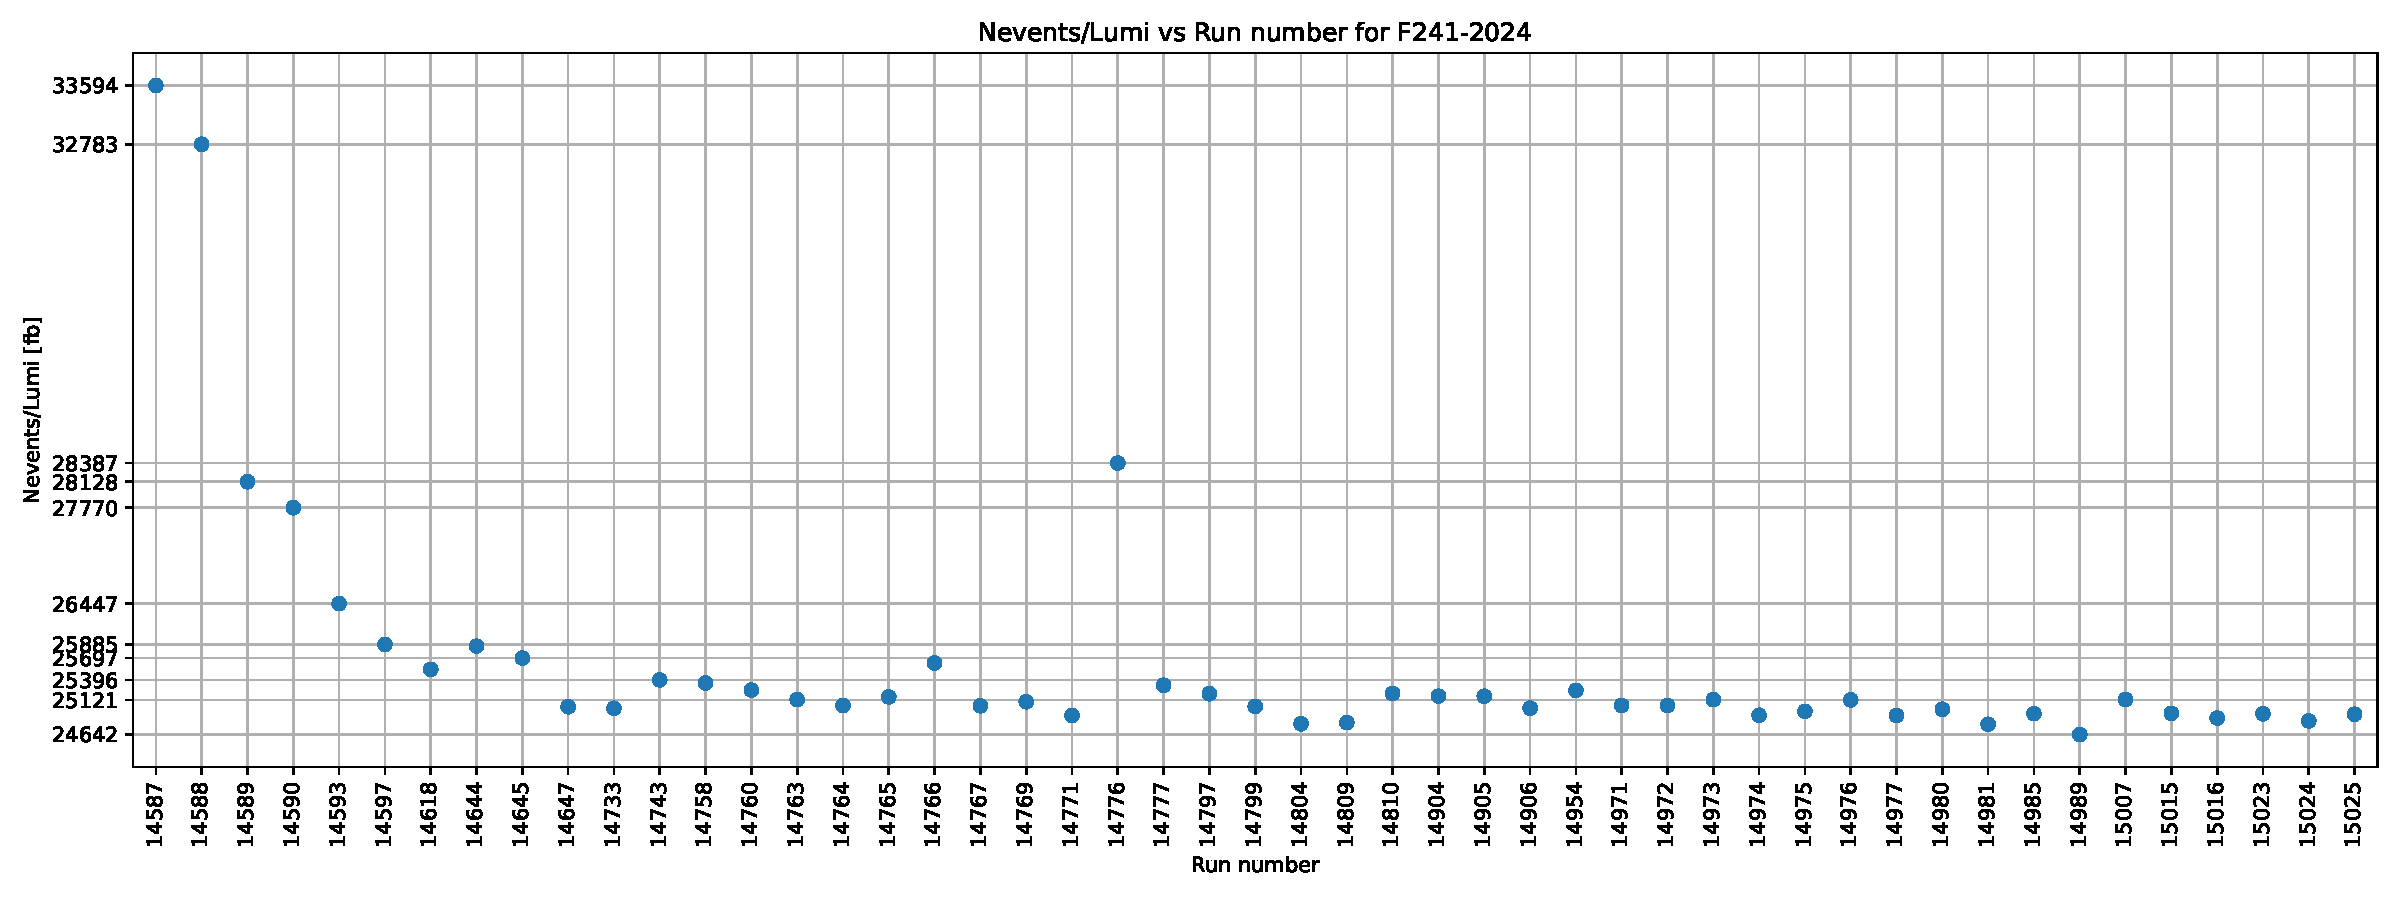
\includegraphics[width=1.0\textwidth]{plots_runwise/NEventsbyLumi_2024_F241.pdf}
    \end{figure}
    \vspace{-0.35cm}
    \begin{figure}
        \centering
        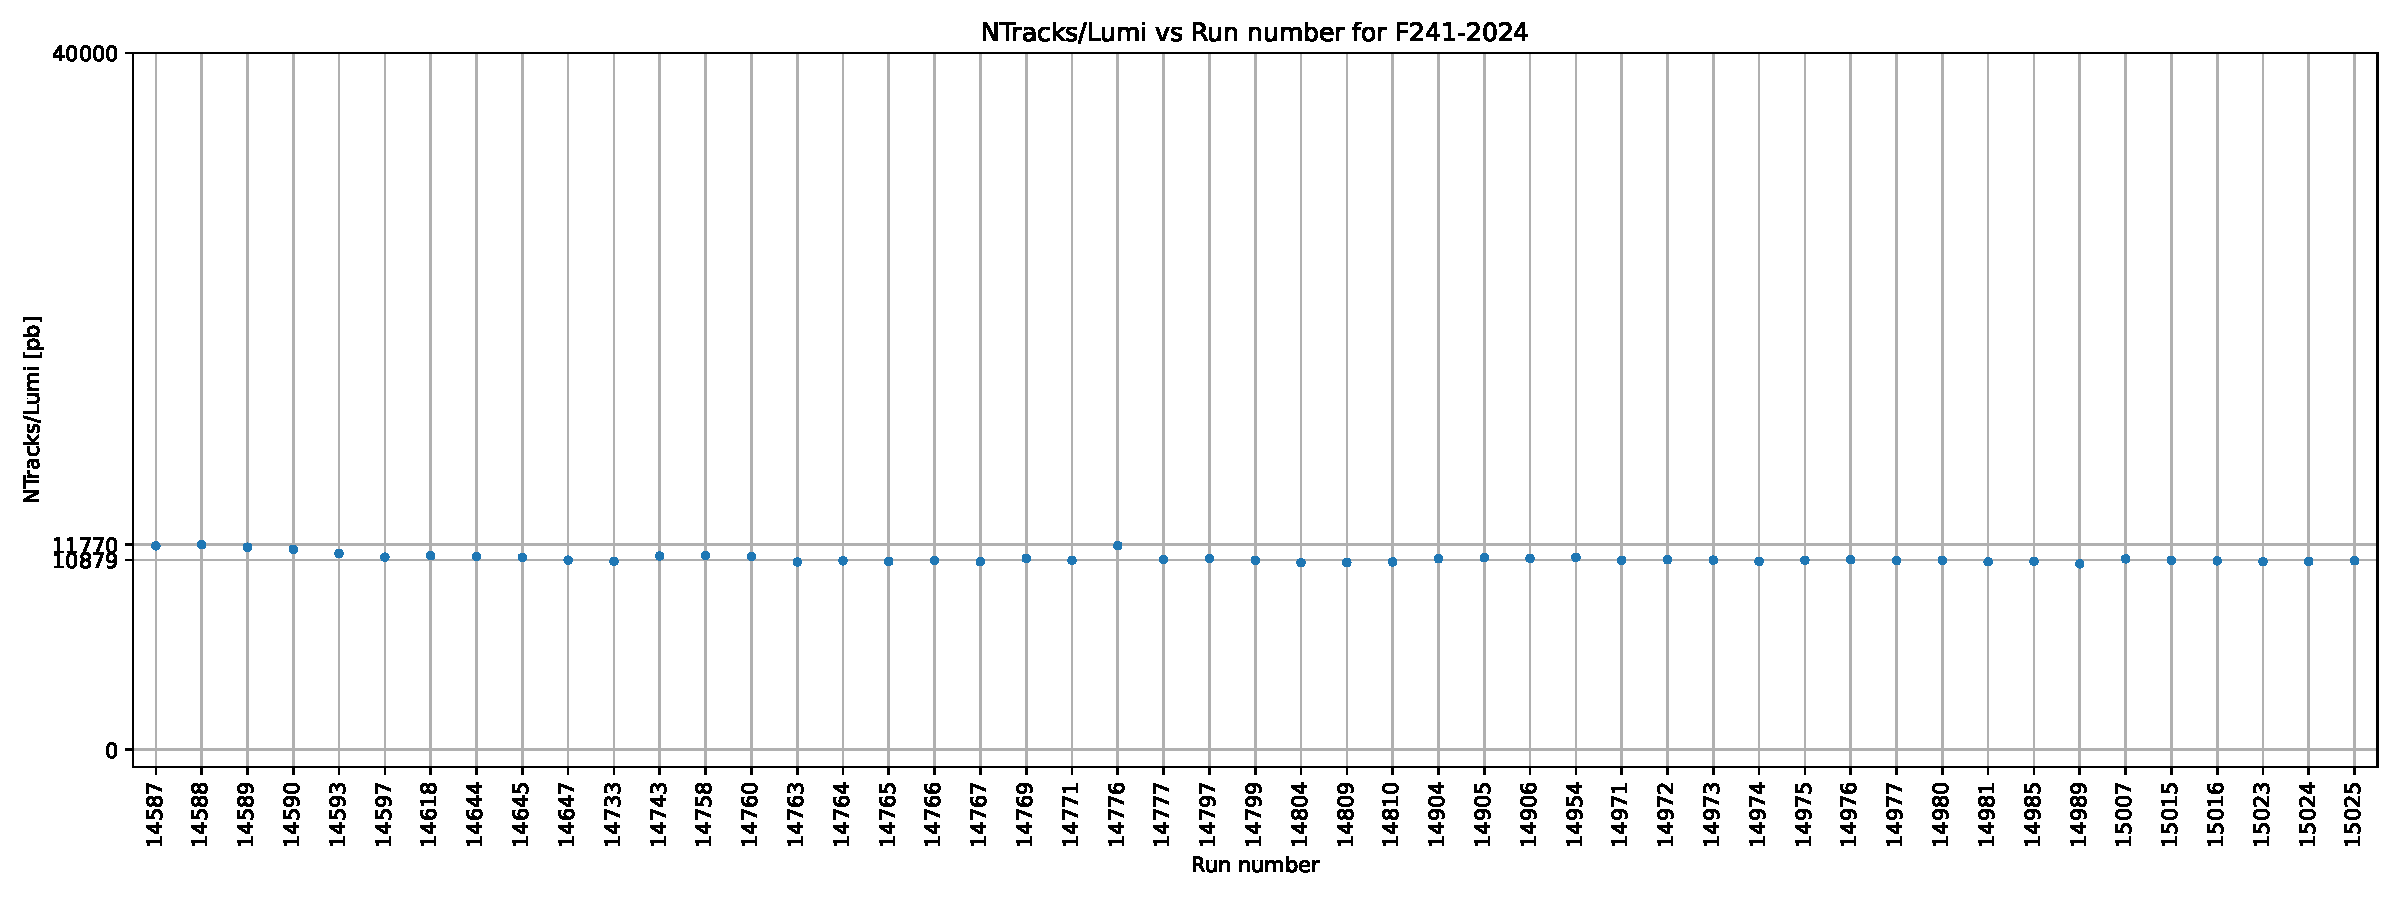
\includegraphics[width=1.0\textwidth]{plots_runwise/NTracksbyLumi_2024_F241.pdf}
    \end{figure}
\end{frame}

\begin{frame}{Runwise Plots of Tungsten only- 2024}
    \begin{figure}
        \centering
        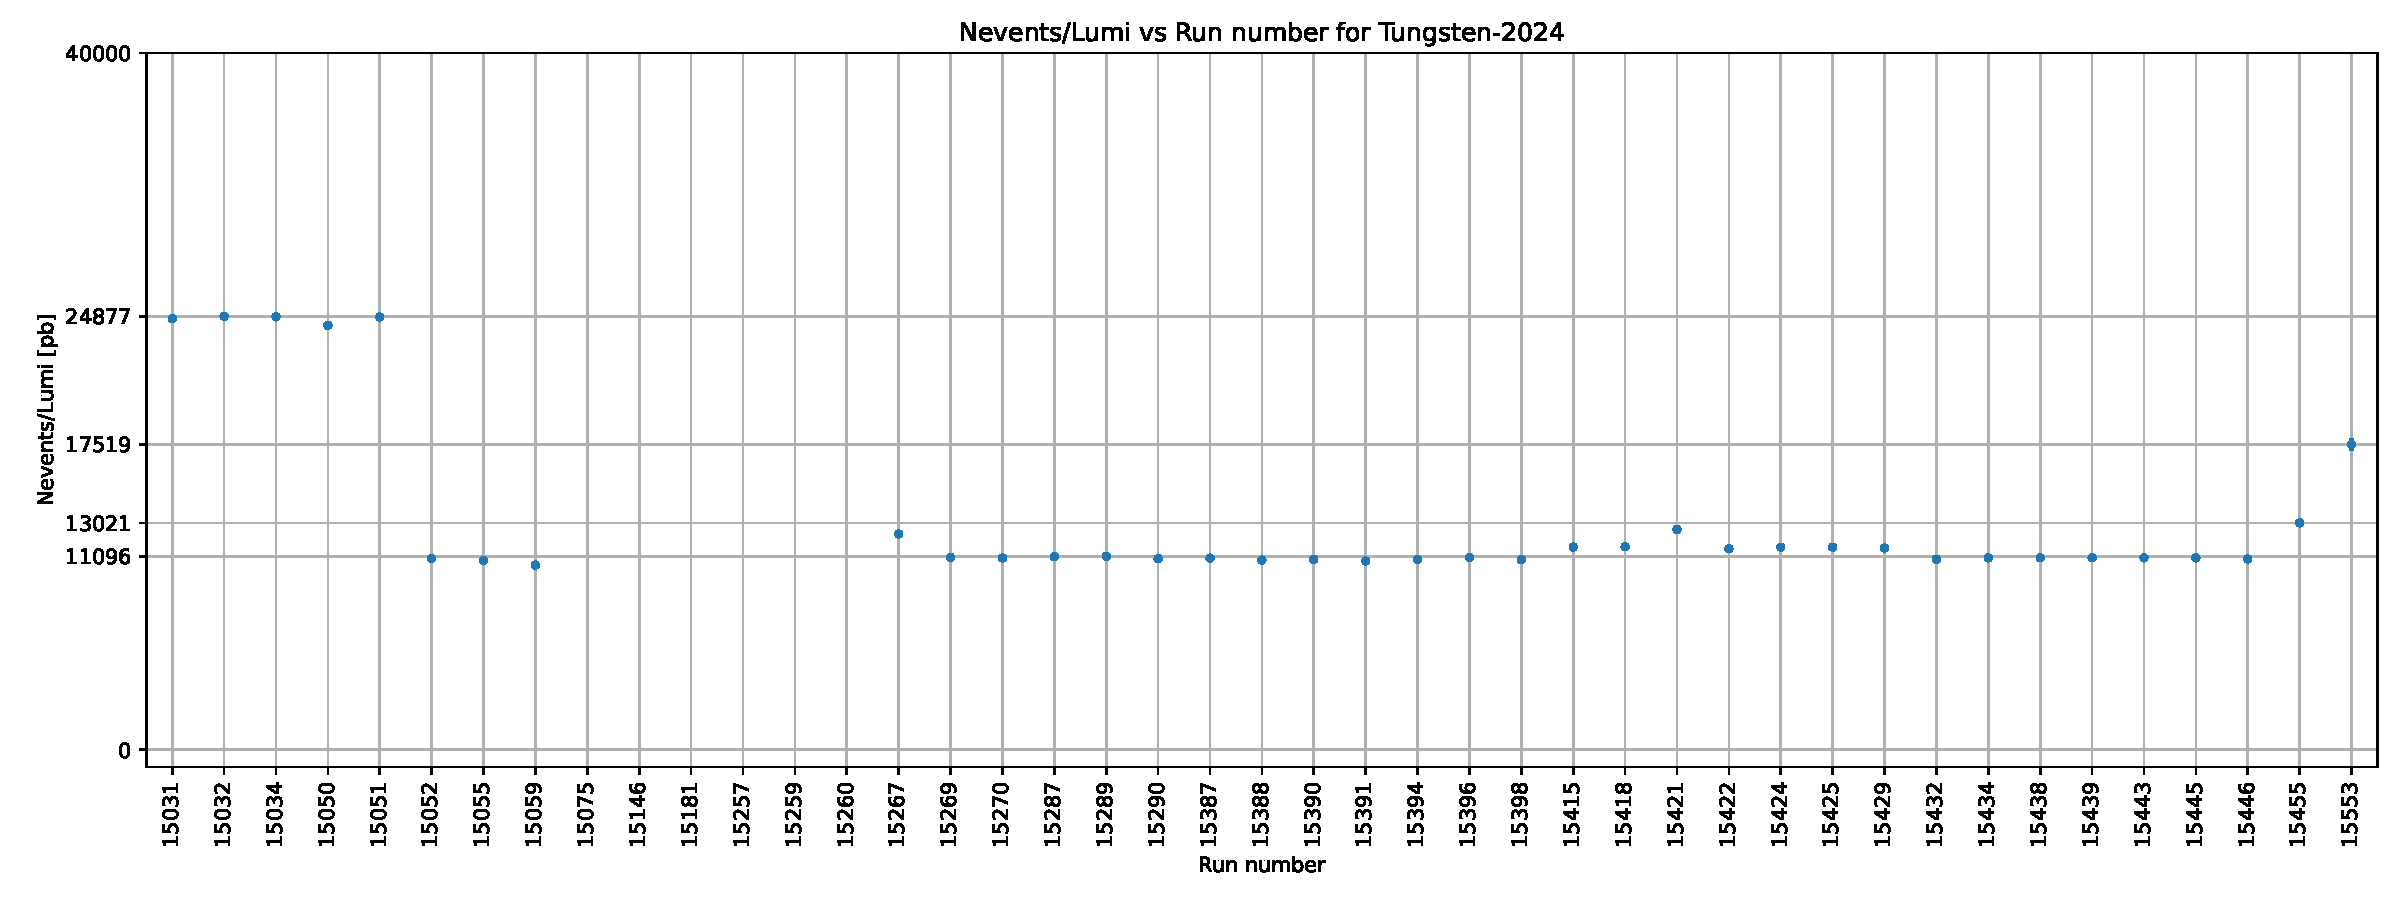
\includegraphics[width=1.0\textwidth]{plots_runwise/NEventsbyLumi_2024_Tungsten.pdf}
    \end{figure}
    \vspace{-0.35cm}
    \begin{figure}
        \centering
        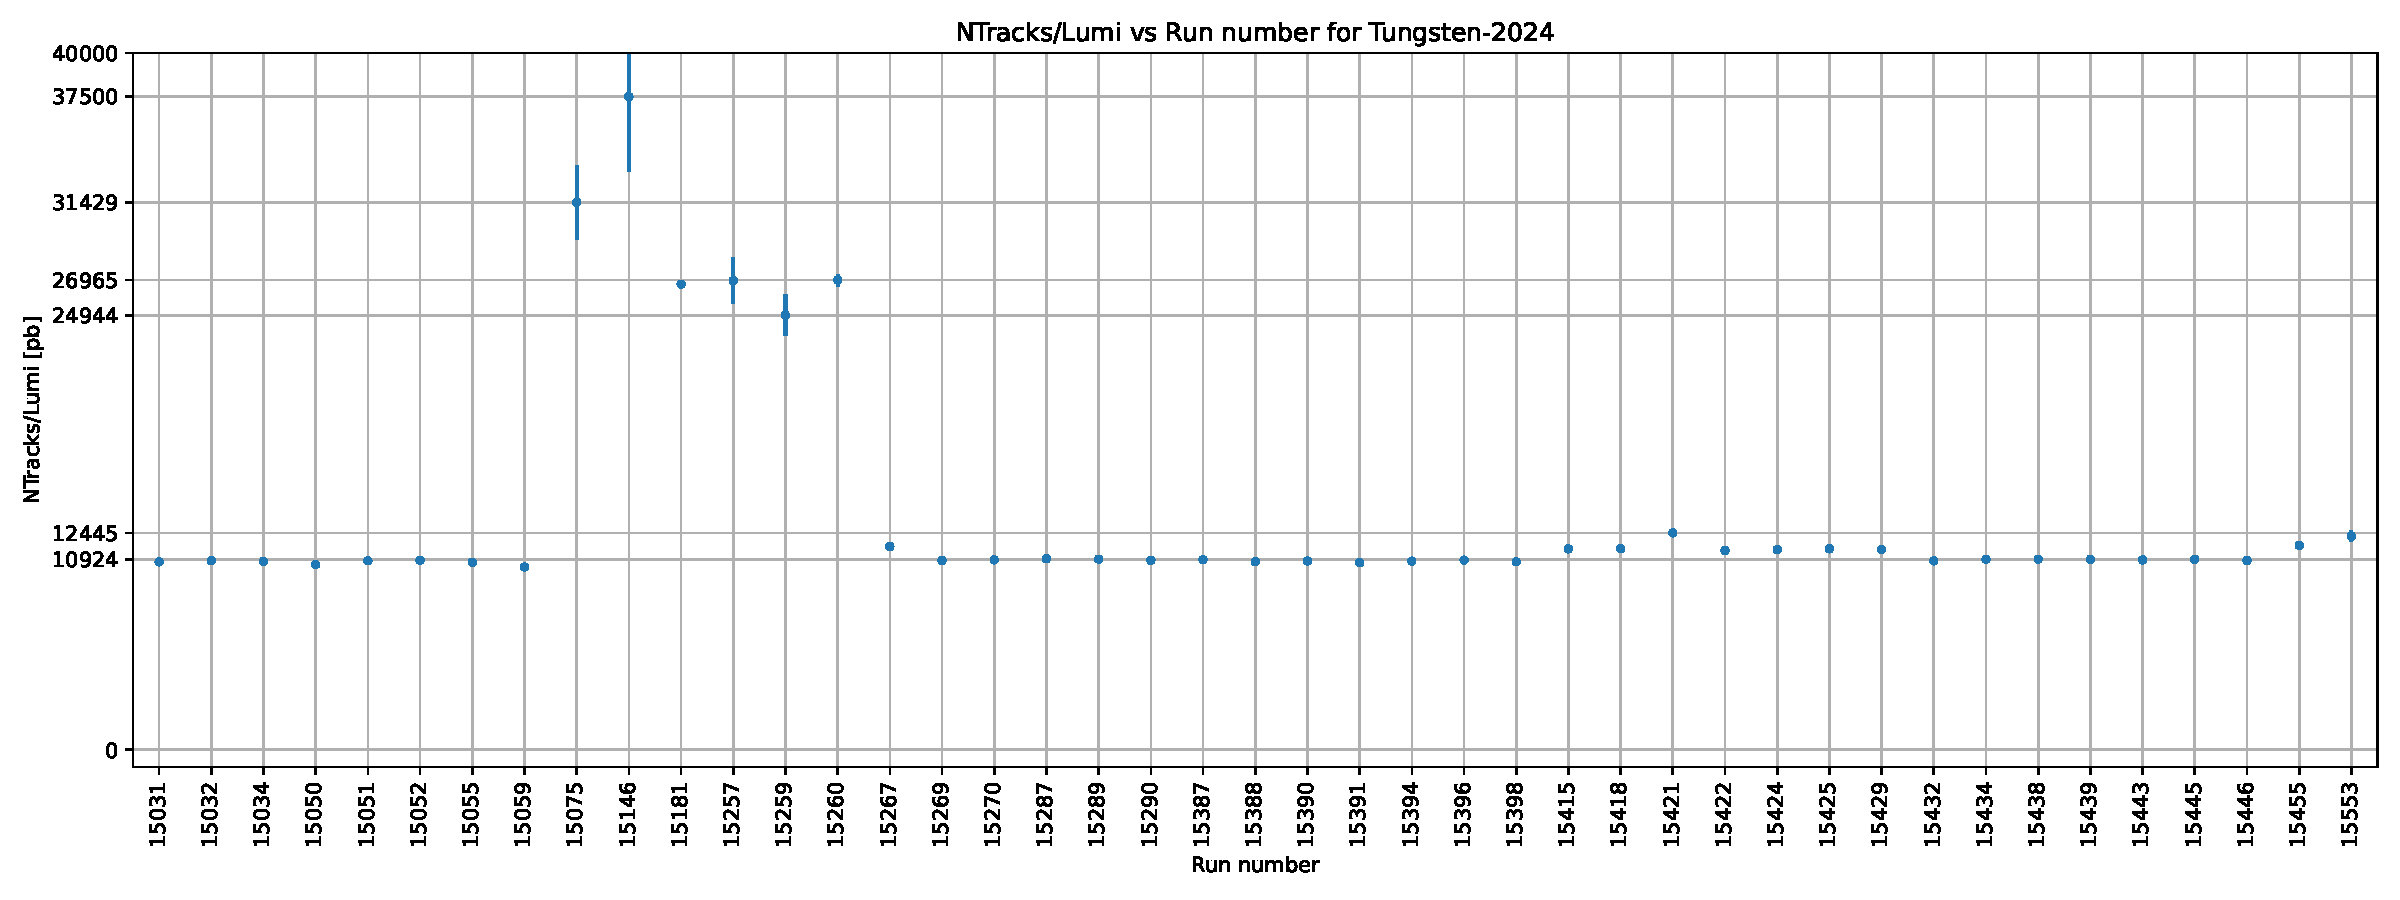
\includegraphics[width=1.0\textwidth]{plots_runwise/NTracksbyLumi_2024_Tungsten.pdf}
    \end{figure}
\end{frame}

\begin{frame}{Runwise Plots of F242- 2024}
    \begin{figure}
        \centering
        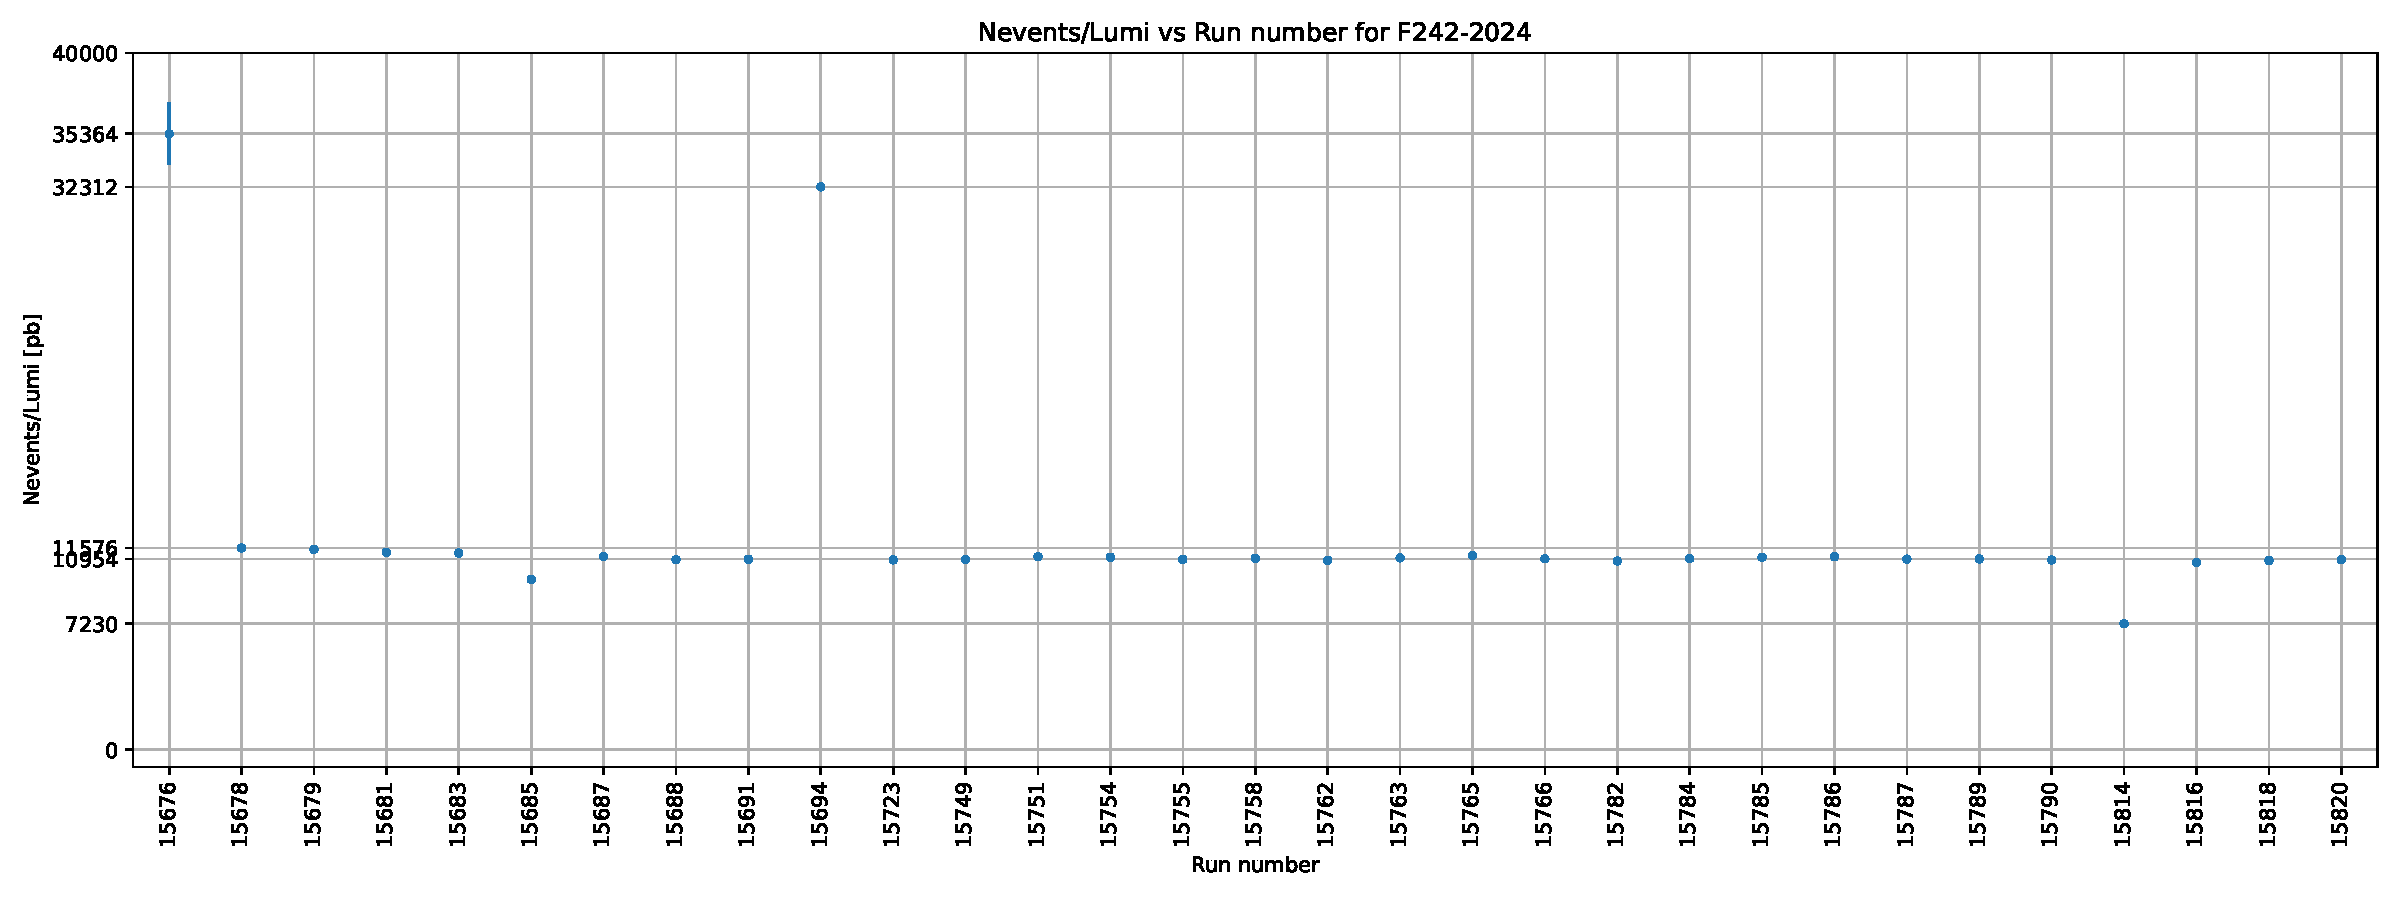
\includegraphics[width=1.0\textwidth]{plots_runwise/NEventsbyLumi_2024_F242.pdf}
    \end{figure}
    \vspace{-0.35cm}
    \begin{figure}
        \centering
        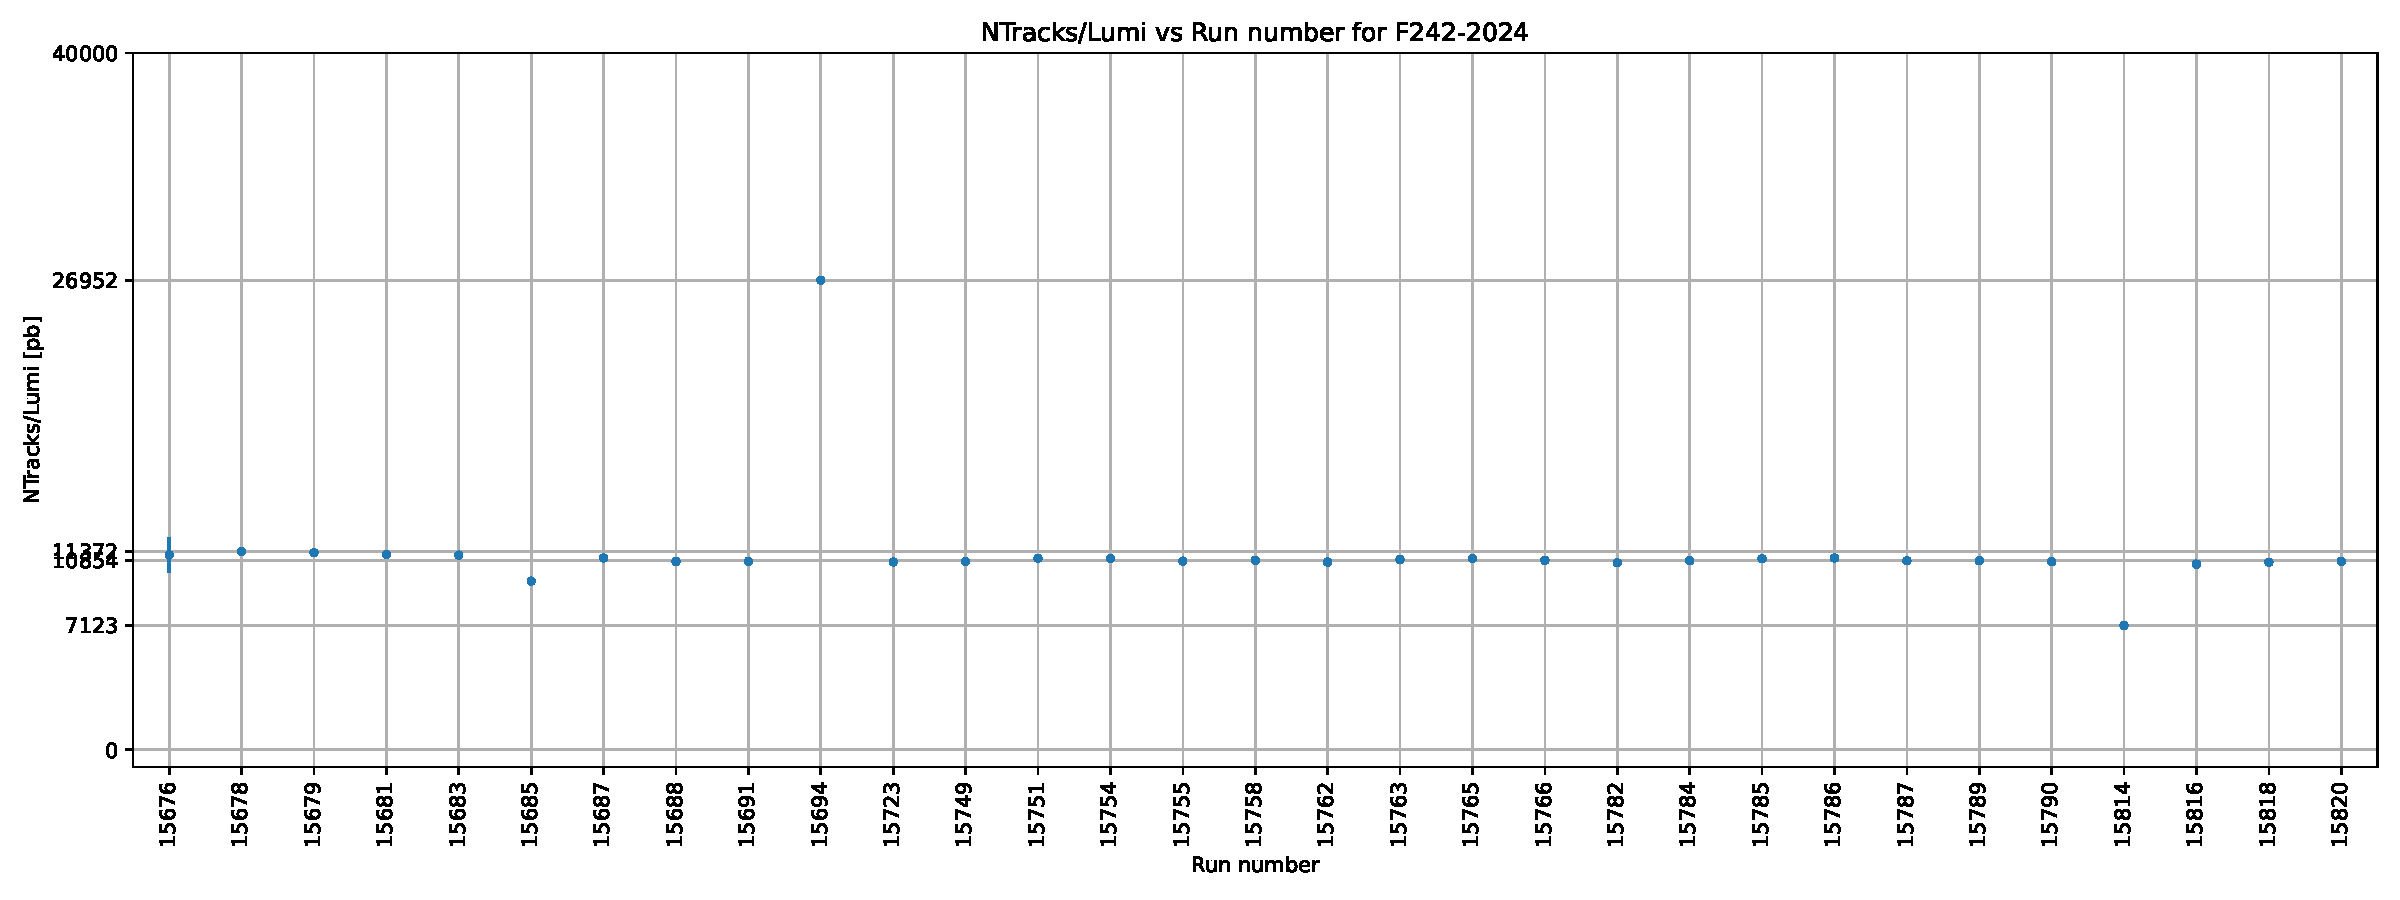
\includegraphics[width=1.0\textwidth]{plots_runwise/NTracksbyLumi_2024_F242.pdf}
    \end{figure}
\end{frame}

\begin{frame}{Runwise Plots of CaloNu - 2024}
    \begin{figure}
        \centering
        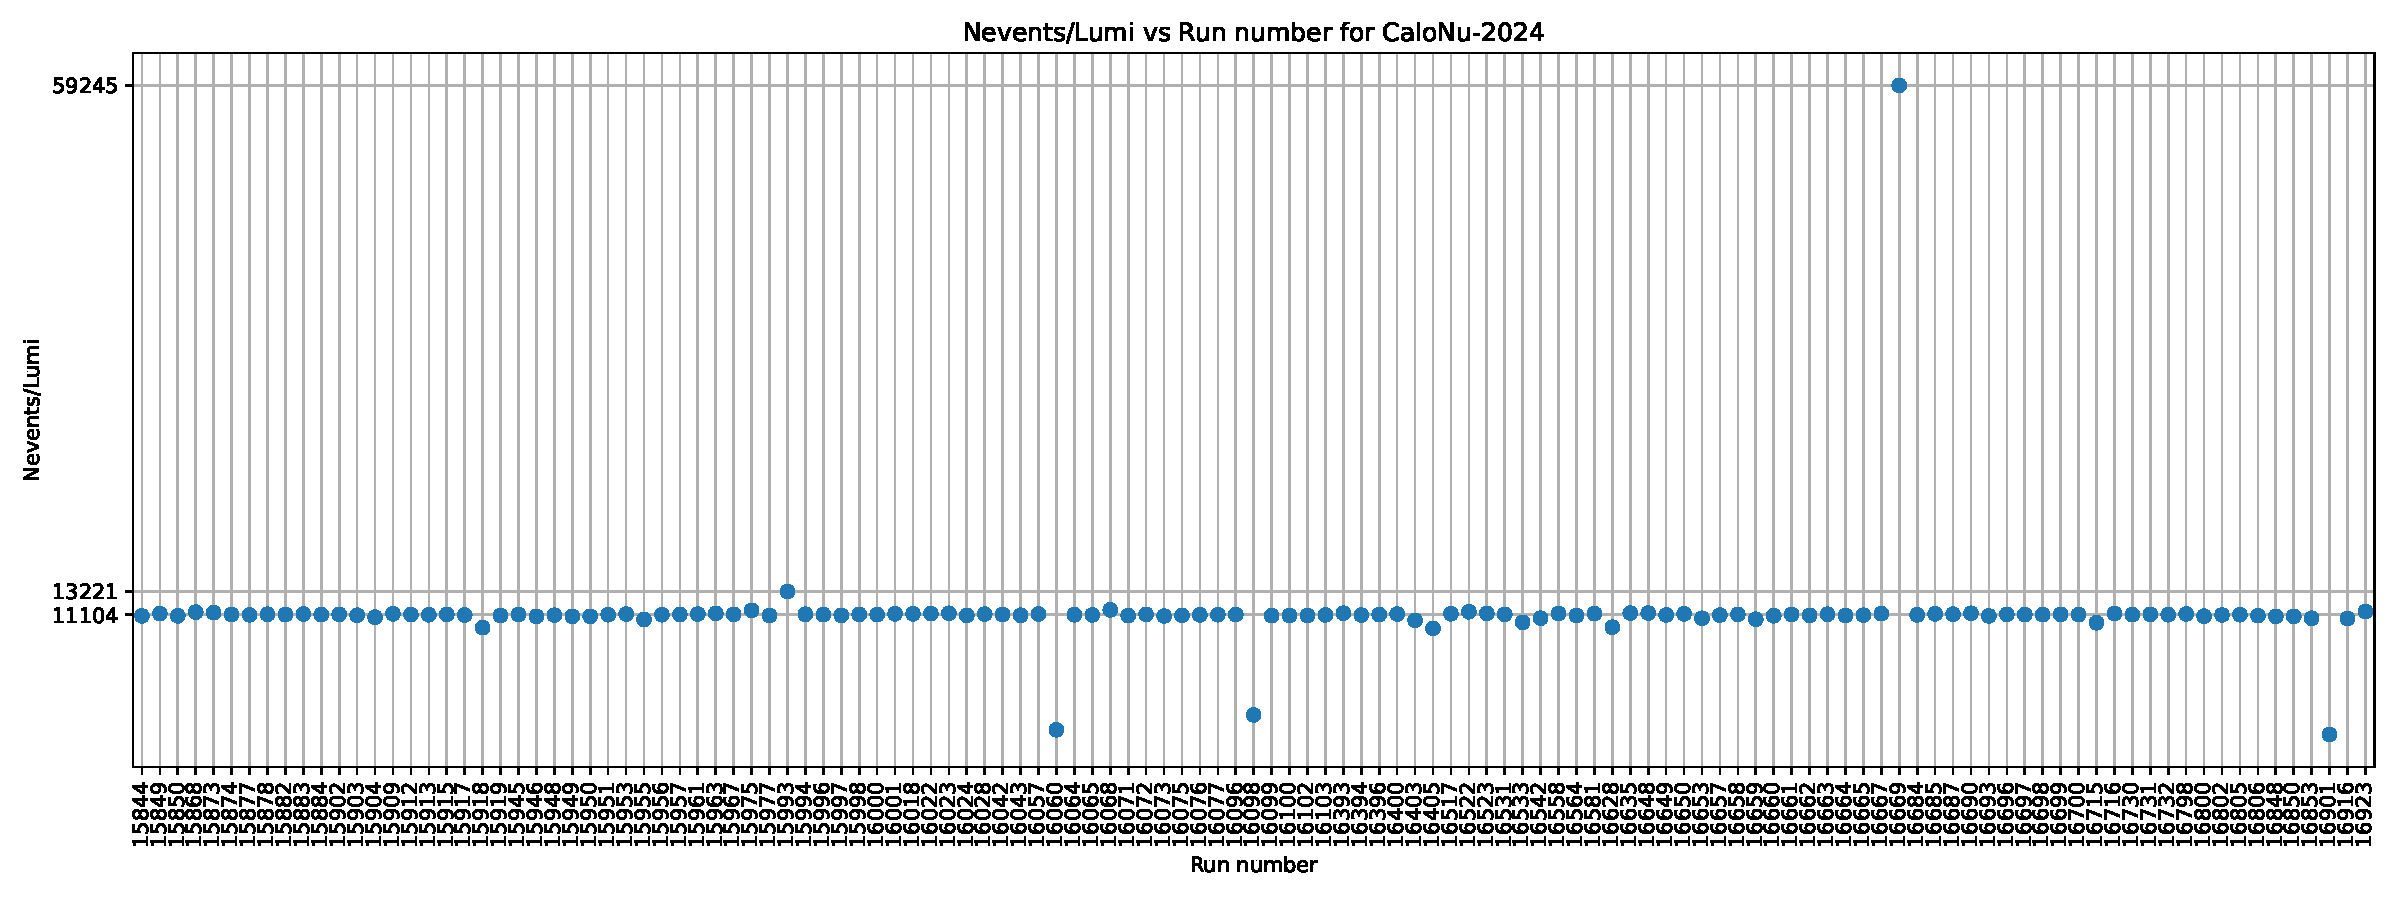
\includegraphics[width=1.0\textwidth]{plots_runwise/NEventsbyLumi_2024_CaloNu.pdf}
    \end{figure}
    \vspace{-0.35cm}
    \begin{figure}
        \centering
        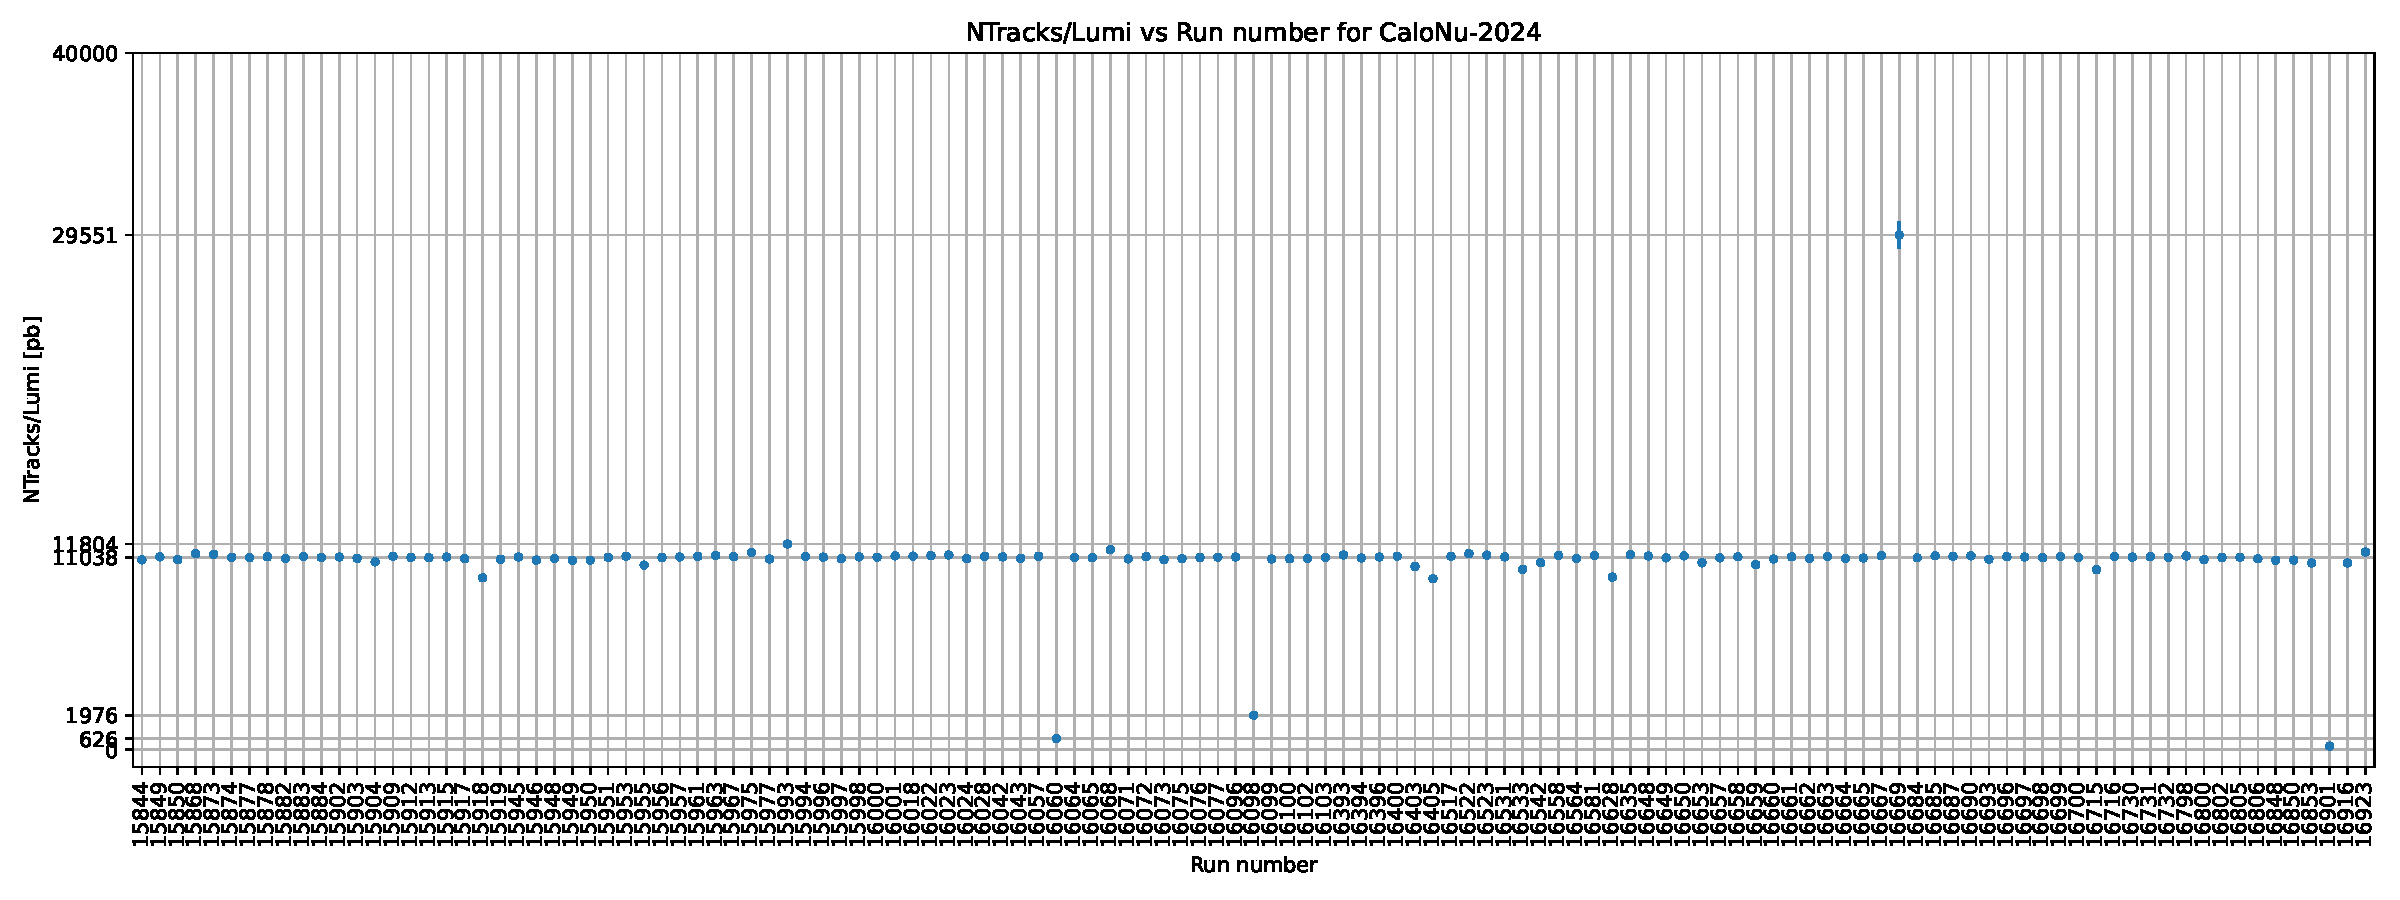
\includegraphics[width=1.0\textwidth]{plots_runwise/NTracksbyLumi_2024_CaloNu.pdf}
    \end{figure}
\end{frame}

\begin{frame}{Runwise Plots of F243- 2024}
    \begin{figure}
        \centering
        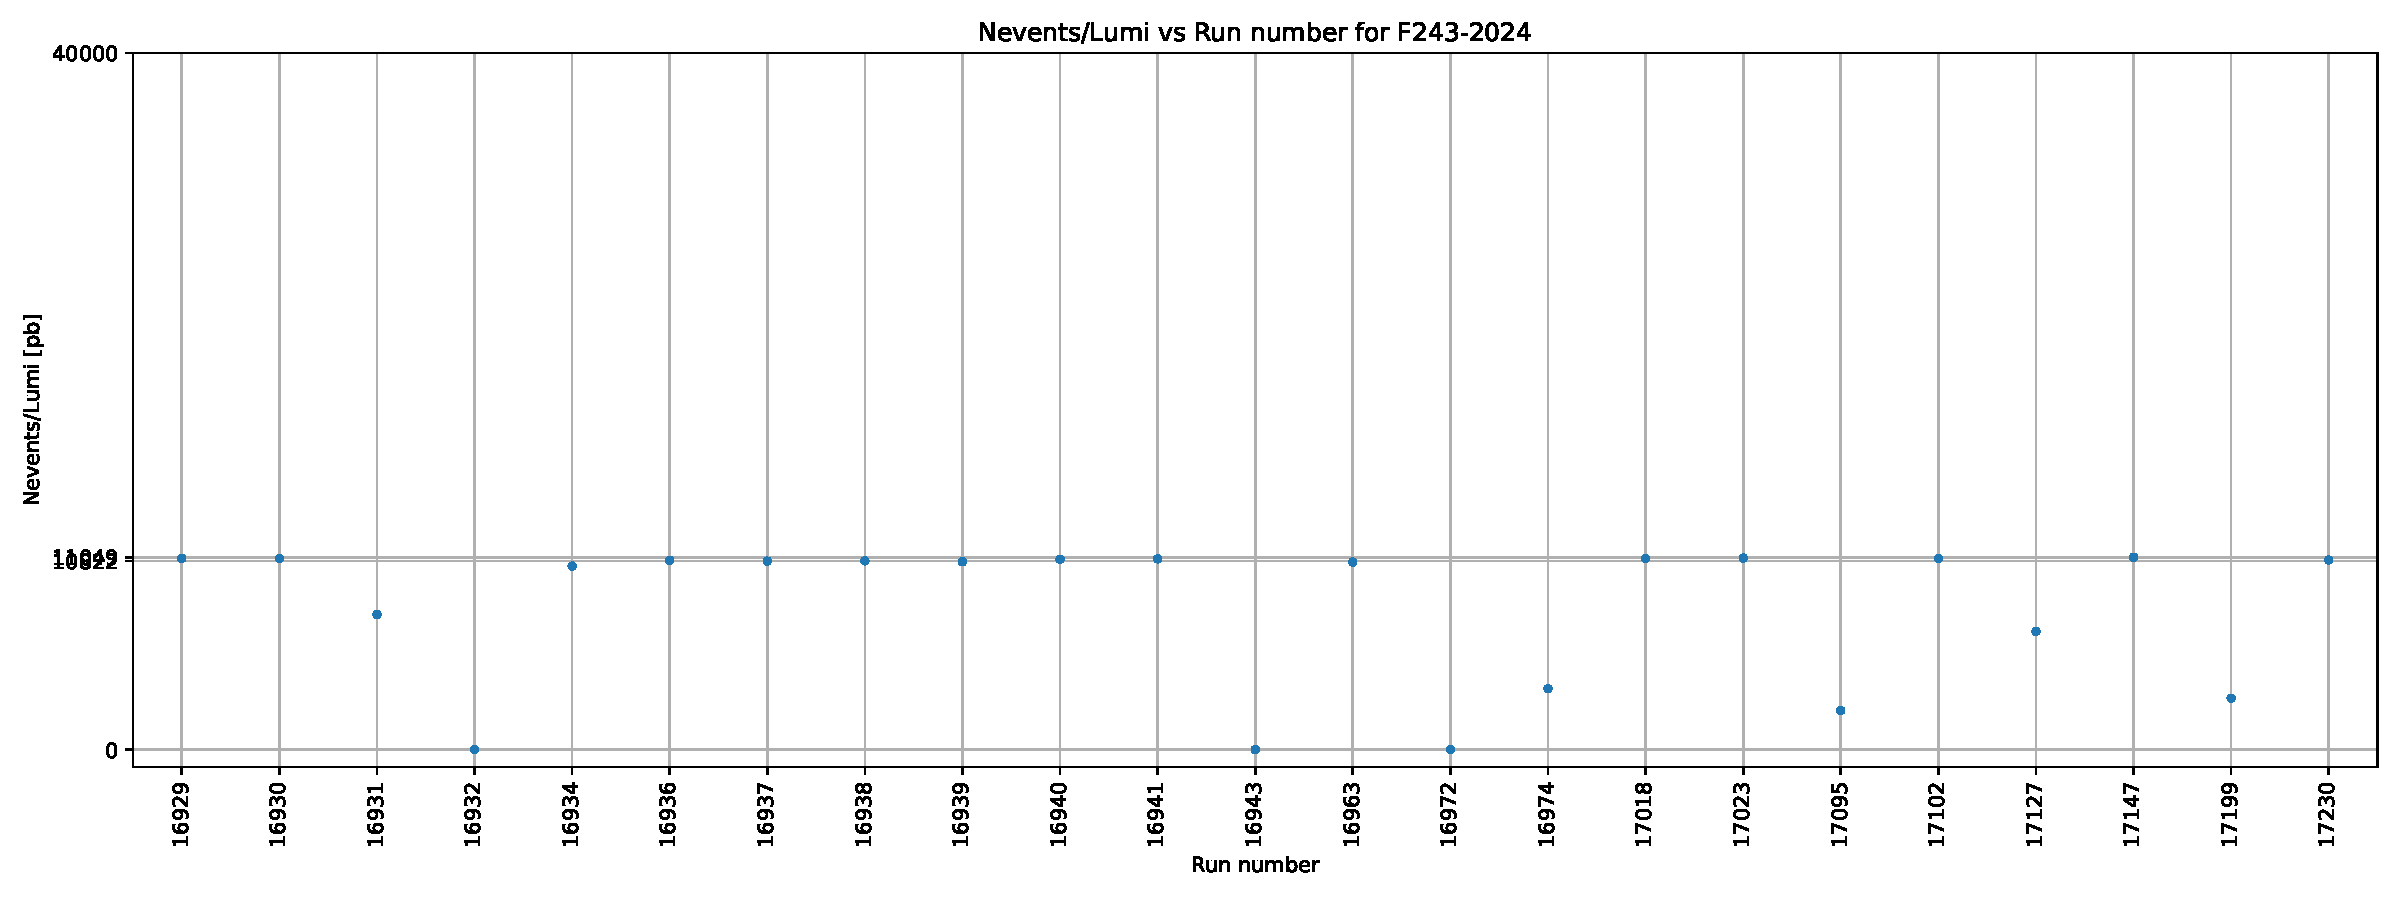
\includegraphics[width=1.0\textwidth]{plots_runwise/NEventsbyLumi_2024_F243.pdf}
    \end{figure}
    \vspace{-0.35cm}
    \begin{figure}
        \centering
        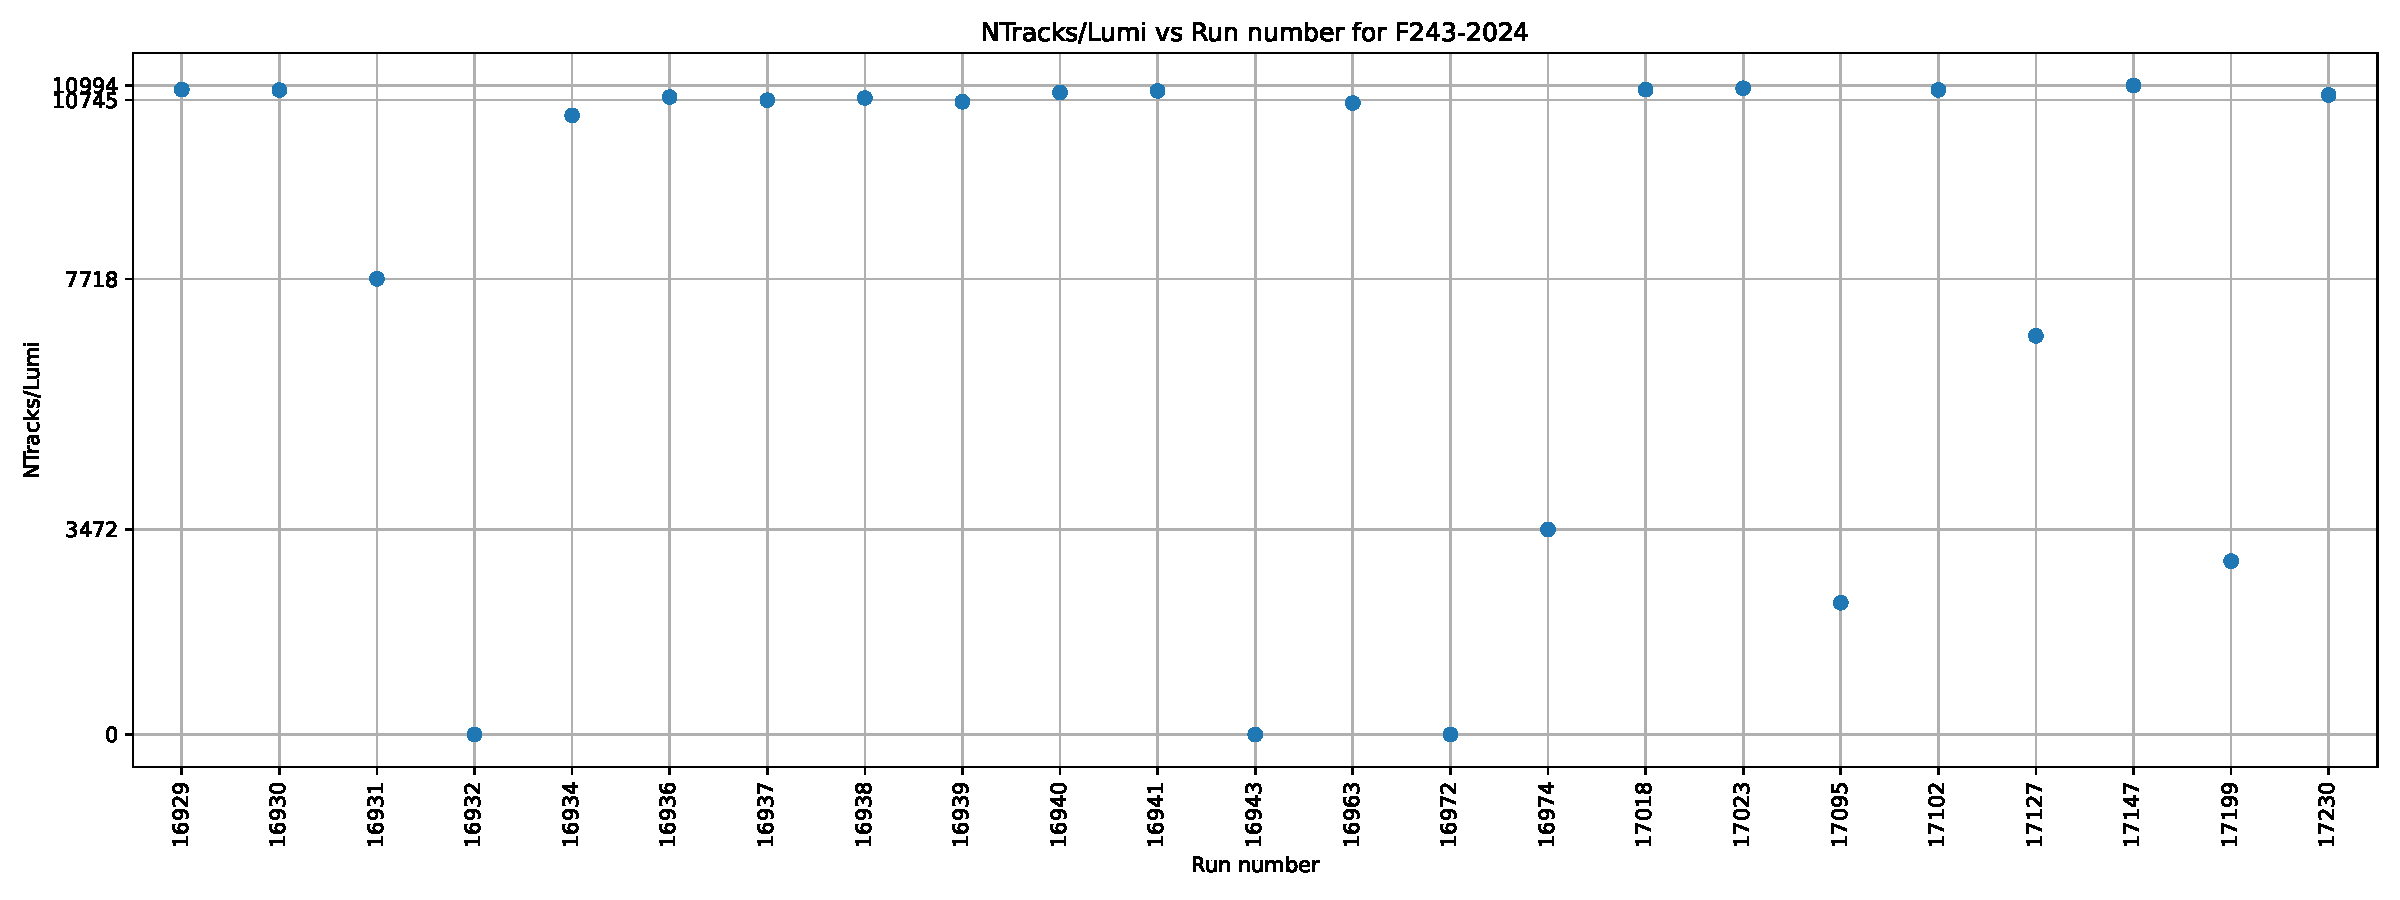
\includegraphics[width=1.0\textwidth]{plots_runwise/NTracksbyLumi_2024_F243.pdf}
    \end{figure}
\end{frame}

\begin{frame}{Micellaneous}
    \begin{itemize}
        \item Similar plots can be made using the \href{https://gitlab.cern.ch/anburger/compareproductions_faser}{compareproductions\_faser} tool.
        \item Link to Repo containing the code for plots in this presentation.
        \item Link to variants of the plots more more filtered like charge separated, good tracks only etc. [Will be Added]
        \item Detailed Runwise plots were presented by Oscar. [See \href{https://indico.cern.ch/event/1476946/contributions/6220240/attachments/2970435/5227381/DQ2024.pdf}{previous DQ Talk}]
    \end{itemize}
    
\end{frame}